\vbtitle{\textbf{Illustrations: Logarithms}}
\BgThispage
\begin{enumerate}
    \item Find the values of the following logarithmic expressions:
        \begin{tasks}(2)
            \task $\log_a a$
            \task $\log_2 8$
            \task $\log_3 81$
            \task $\log(1)$
            \task $\log_{10} 2$
            \task $\log_{10} 3$
            \task $\log_{10} 6$
            \task $\log_{10} 5$
        \end{tasks}
        \begin{solution}
            \begin{multicols}{2}
            \begin{enumerate}
                \item 
                    \begin{align*}
                        \text{Let, \quad}\log_a a &= x\\
                        a &= a^x\\
                        x &= 1\\
                        \Aboxed{\log_a a &= 1}
                        \intertext{If base and argument are the same, the value of the logarithm is 1.}
                    \end{align*}

                \item 
                    \begin{align*}
                        \log_2 8 &= \log_2 2^3\\
                        &= 3\log_2 2\\
                        &= 3
                    \end{align*}

                \item 
                    \begin{align*}
                        \log_3 81 &= \log_3 3^4\\
                        &= 4\log_3 3\\
                        &= 4
                    \end{align*}

                \item
                    \begin{align*}
                        \log(1) &= x\\
                        \intertext{Here, we have no particular base, so we can assume the base to be 10, but it can be any base, so lets say the base is \( b \).}
                        1 &= b^x\\
                        \intertext{It doesn't matter what the value of $b(\neq 0)$ is, $x$ has to be zero.}
                        x &= 0\\
                        \Aboxed{\log_{\textit{any base}}(1) &= 0}
                    \end{align*}

                \item
                    \begin{align*}
                        &\log_{10} 2\\
                        \intertext{Actually, we can find it using some expansion series or by looking log table, but right now we will try to approximate it.}
                        2^3 &= 9, \quad 2^4 = 16\\
                        2^{3.3} &\approx 10\\
                       \Rightarrow &\log_{2^{3.3}} 2\\
                       &= \frac{1}{3.3}\log_2 2\\
                          &= \frac{1}{3.3}\\
                            &\approx 0.3
                        \intertext{Again, this method won't give us the exact value, but we can reach close to it pretty easily.}
                    \end{align*}

                \item
                    \begin{align*}
                        &\log_{10} 3\\
                        3^2 &= 9, \quad 3^3 = 27\\
                        3^{2.1} &\approx 10\\
                    \end{align*}
                    \begin{center}
                        \begin{tikzpicture}
                            \tzline(0, 0)(5, 0)
                            \tzticks*{0, 0.5, 1, 1.5, 2, 2.5, 3, 3.5, 4, 4.5, 5}
                            \tzticks{0/$9$, 5/$27$}
                            \tzticks<0, 0.6>{0/$2$, 5/$3$}
                        \end{tikzpicture}
                    \end{center}
                    \begin{align*}
                        \Rightarrow &\log_{3^{2.1}} 3\\
                        &= \frac{1}{2.1}\log_3 3\\
                        &= \frac{1}{2.1}\\
                        &\approx 0.47
                    \intertext{Again, it's not the exact value, but it's very close to it.}
                    \end{align*}

                \item
                    \begin{align*}
                        &\log_{10} 6\\
                        &=\log_{10} 2 + \log_{10} 3\\
                        &\approx 0.3 + 0.47\\
                        &\approx 0.77
                    \end{align*}

                \item
                    \begin{align*}
                        &\log_{10} 5\\
                        &= \log_{10} 10 - \log_{10} 2\\
                        &= 1 - 0.3\\
                        &= 0.7
                    \end{align*}
            \end{enumerate}
            \end{multicols}
        \end{solution}
    \item Find the value of x satisfying the equation \[ \log_3(5+4\log_3(x-1))=2.\]
        \begin{solution}
            \begin{align*}
                \intertext{Just apply the conversion from log to exponential form.}
                \log_3(5+4\log_3(x-1)) &= 2\\
                5+4\log_3(x-1) &= 3^2\\
                5+4\log_3(x-1) &= 9\\
                4\log_3(x-1) &= 4\\
                \log_3(x-1) &= 1\\
                x-1 &= 3\\
                x &= 4
            \end{align*}
        \end{solution}

        \BgThispage
    \item Solve for x: $5^{\log_{10}x}=50-x^{\log_{10}5}$.
        \begin{solution}
            \begin{align*}
                \intertext{Apply $a^{\log_b c} = c^{\log_b a}$}
                5^{\log_{10}x} &= 50-x^{\log_{10}5}\\
                5^{\log_{10}x} &= 50-\left(5^{\log_{10}x}\right)\\
                5^{\log_{10}x} &= 50-5^{\log_{10}x}\\
                2\cdot 5^{\log_{10}x} &= 50\\
                5^{\log_{10}x} &= 25\\
                \log_{10}x &= 2\\
                x &= 10^2\\
                x &= 100
            \end{align*}
        \end{solution}

    \item Solve for x: $1+\log_2(x-1)=\log_{(x-1)}4$.
        \begin{solution}
            \begin{align*}
                1 + \log_2(x-1) &= \log_{(x-1)}4\\
                1 + \log_2(x-1) &= \frac{\log_2 4}{\log_2 (x-1)}\\
                1 + \log_2(x-1) &= \frac{2}{\log_2 (x-1)}\\
                \intertext{Let \( \log_2 (x-1) = t \)}
                1 + t &= \frac{2}{t}\\
                t^2 + t - 2 &= 0\\
                (t+2)(t-1) &= 0\\
                t &= -2, 1\\
                \log_2 (x-1) &= 1, \qquad \log_2 (x-1) = -2\\
                x-1 &= 2, \qquad x-1 = 2^{-2}\\
                x &= 3, \qquad x = \frac{1}{4} + 1\\
                x &= 3, \qquad x = \frac{5}{4}
            \end{align*}
            \vbstarednote{Sometimes you have to check the solutions to see if they are valid, by substituting them back into the original equation.}
        \end{solution}
        \BgThispage

\end{enumerate}